% ------------------------------------------------------------------------
% ------------------------------------------------------------------------
% Monografia Device Aware Building
% Trabalho de Conclusão de Curso
% Baseia-se no documento modelo de TCC do abntex2
% Para saber mais, acesse https://github.com/abntex/abntex2
% ------------------------------------------------------------------------
% ------------------------------------------------------------------------

\documentclass[
	% -- opções da classe memoir --
	12pt,				% tamanho da fonte
	openright,			% capítulos começam em pág ímpar (insere página vazia caso preciso)
	oneside,			% para impressão em verso e anverso. Oposto a oneside
	a4paper,			% tamanho do papel.
	% -- opções da classe abntex2 --
	chapter=TITLE,		% títulos de capítulos convertidos em letras maiúsculas
	%section=TITLE,		% títulos de seções convertidos em letras maiúsculas
	%subsection=TITLE,	% títulos de subseções convertidos em letras maiúsculas
	%subsubsection=TITLE,% títulos de subsubseções convertidos em letras maiúsculas
	% -- opções do pacote babel --
	english,			% idioma adicional para hifenização
	brazil				% o último idioma é o principal do documento
	]{abntex2}


% ----------------------------------------------------------
% Pacotes básicos
% ----------------------------------------------------------
%\usepackage{helvet}
\usepackage[scaled]{helvet}
\renewcommand*\familydefault{\sfdefault}	% Only if the base font of the document is to be sans serif (by Gabriel Oliveira)
\usepackage[T1]{fontenc}	% Selecao de codigos de fonte.
\usepackage[utf8]{inputenc}	% Codificacao do documento (conversão automática dos acentos)
\usepackage{lastpage}		% Usado pela Ficha catalográfica
\usepackage{indentfirst}	% Indenta o primeiro parágrafo de cada seção.
\usepackage{color}			% Controle das cores
\usepackage{graphicx}		% Inclusão de gráficos
\usepackage{microtype}		% para melhorias de justificação
% ----------------------------------------------------------


% ----------------------------------------------------------
% Pacotes adicionais, usados apenas no âmbito do Modelo Canônico do abnteX2
%% ----------------------------------------------------------
% \usepackage{lipsum}				% para geração de dummy text
\usepackage{000-sty/customizacoes}		% customizações feitas pelo autor
% ----------------------------------------------------------

% ----------------------------------------------------------
% Pacotes de citações
% ----------------------------------------------------------
\usepackage[brazilian,hyperpageref]{backref}	% Paginas com as citações na bibl
\usepackage[alf]{abntex2cite}					% Citações padrão ABNT

% ----------------------------------------------------------
% CONFIGURAÇÕES DE PACOTES
% ----------------------------------------------------------

% ----------------------------------------------------------
% Configurações do pacote backref
% ----------------------------------------------------------
\definecolor{thered}{rgb}{0.65,0.04,0.07}
\definecolor{thegreen}{rgb}{0.06,0.44,0.08}
\definecolor{thegrey}{gray}{0.5}
\definecolor{theshade}{rgb}{1,1,0.97}
\definecolor{theframe}{gray}{0.6}
% ----------------------------------------------------------

% Usado sem a opção hyperpageref de backref
\renewcommand{\backrefpagesname}{ }
% Texto padrão antes do número das páginas
\renewcommand{\backref}{\ABNTEXchapterfont}
% Define os textos da citação


% ----------------------------------------------------------
% Informações de dados para CAPA e FOLHA DE ROSTO
% ----------------------------------------------------------

\titulo{Habilitando um Prédio a Localizar Contextualmente Dispositivos utilizando Redes Sem Fio}
\autor{Luís Henrique Puhl de Souza}
\local{Bauru}
\data{2016}
\orientador{Prof. Dr. Eduardo Martins Morgado}

% O preambulo deve conter o tipo do trabalho, o objetivo,
% o nome da instituição e a área de concentração
% foi necessário utilizar \~{a} e etc para os acentos por problemas na geração do PDF

\instituicao{%
 Universidade Estadual Paulista ``Júlio de Mesquita Filho''
 \par
 Faculdade de Ciências - Campus Bauru
 \par
 Departamento de Computação
}

\tipotrabalho{Monografia (Trabalho de Conclusão de Curso)}

\preambulo{Trabalho de Conclus\~{a}o do Curso de Bacharelado em Ci\^{e}ncia da
Computa\c{c}\~{a}o apresentado ao Departamento de Computa\c{c}\~{a}o da
Faculdade de Ci\^{e}ncias da Universidade Estadual Paulista ``J\'{ú}lio de
Mesquita Filho'' – UNESP, C\^{a}mpus de Bauru.}

% ----------------------------------------------------------
% Configurações de projeto
% ----------------------------------------------------------
% MODIFICA A APRESENTACAO DAS PARTES OPCIONAIS
% ----------------------------------------------------------
% PARTE EXTERNA
%	Capa				(obrigatorio)
%	*Lombada			(opcional)
\newif\iflombada
\lombadafalse
% ELEMENTOS PRE-TEXTUAIS
%	Folha de rosto		(obrigatorio)
%	*Ficha Catalografica	(opcional) (obrigatoria para a UNESP-FC-BAURU)
\newif\ifficha
\fichatrue
%	*Errata			(opcional)
\newif\iferrata
\erratafalse
%	Folha Aprovacao		(obrigatorio)
%	*Dedicatoria		(opcional)
\newif\ifdedicatoria
\dedicatoriafalse
%	*Agradecimentos		(opcional)
\newif\ifagradecimentos
\agradecimentosfalse
%	*Epigrafe			(opcional)
\newif\ifepigrafe
\epigrafefalse
%	Resumo				(obrigatorio)
\newif\ifresumo
\resumotrue
%	Resumo ingles		(obrigatorio)
%	*Lista Ilustracoes	(opcional)
\newif\iffiguras
\figurasfalse
%	*Lista Tabelas		(opcional)
\newif\iftabelas
\tabelasfalse
%	*Lista Abreviaturas	(opcional)
\newif\ifabreviaturas
\abreviaturasfalse
%	*Lista Simbolos		(opcional)
\newif\ifsimbolos
\simbolosfalse
%	Sumario				(obrigatorio)
% ELEMENTOS TEXTUAIS
%	Introducao
%	Desenvolvimento		(capitulos e subcapitulos)
%	Conclusao
% ELEMENTOS POS-TEXTUAIS
%	Referencias			(obrigatorio)
%	*Glossario			(opcional)
\newif\ifglossario
\glossariofalse
%	*Apendice			(opcional)
\newif\ifapendice
\apendicefalse
%	*Anexo				(opcional)
\newif\ifanexo
\anexofalse
%	*Indice		(opcional)
\newif\ifindice
\indicefalse
% ----------------------------------------------------------

% ----------------------------------------------------------
% Configurações de aparência do PDF final
% ----------------------------------------------------------

% alterando o aspecto da cor azul
\definecolor{blue}{RGB}{0,0,0}

% informações do PDF
\makeatletter
\hypersetup{
		%pagebackref=true,
		pdftitle={\@title},
		pdfauthor={\@author},
		pdfsubject={\imprimirpreambulo},
		pdfcreator={LaTeX with abnTeX2},
		pdfkeywords={iot}{raspberry pi}{internet das coisas}{abntex2}{trabalho acadêmico},
		colorlinks=true,			% false: boxed links; true: colored links
		linkcolor=blue,			% color of internal links
		citecolor=blue,				% color of links to bibliography
		filecolor=magenta,			% color of file links
		urlcolor=blue,
		bookmarksdepth=4
}
\makeatother
% ----------------------------------------------------------

% ----------------------------------------------------------
% Espaçamentos entre linhas e parágrafos
% ----------------------------------------------------------

% O tamanho do parágrafo é dado por:
\setlength{\parindent}{1.3cm}

% Controle do espaçamento entre um parágrafo e outro:
\setlength{\parskip}{0.2cm} % tente também \onelineskip

% ----------------------------------------------------------
% compila o indice
% ----------------------------------------------------------
\makeindex
% ----------------------------------------------------------


% ----------------------------------------------------------


% ----------------------------------------------------------
% Início do documento
% ----------------------------------------------------------
\begin{document}

% Seleciona o idioma do documento (conforme pacotes do babel)
%\selectlanguage{english}
\selectlanguage{brazil}

% Retira espaço extra obsoleto entre as frases.
\frenchspacing

% ----------------------------------------------------------
% ELEMENTOS PRÉ-TEXTUAIS
% ----------------------------------------------------------
\pretextual


% ----------------------------------------------------------
% Capa
% ----------------------------------------------------------
\imprimircapa
% ----------------------------------------------------------


% ----------------------------------------------------------
% Folha de rosto
% (o * indica que haverá a ficha bibliográfica)
% ----------------------------------------------------------
\imprimirfolhaderosto
% ----------------------------------------------------------


% ----------------------------------------------------------
% Inserir a ficha catalográfica
% ----------------------------------------------------------

% Isto é um exemplo de Ficha Catalográfica, ou "Dados internacionais de
% catalogação-na-publicação''. Você pode utilizar este modelo como referência.
% Porém, provavelmente a biblioteca da sua universidade lhe fornecerá um PDF
% com a ficha catalográfica definitiva após a defesa do trabalho. Quando estiver
% com o documento, salve-o como PDF no diretório do seu projeto e substitua todo
% o conteúdo de implementação deste arquivo pelo comando abaixo:
%
% \begin{fichacatalografica}
%	\includepdf{fig_ficha_catalografica.pdf}
% \end{fichacatalografica}

\ifficha
 \begin{fichacatalografica}
	\sffamily
	\vspace*{\fill}					% Posição vertical
	\begin{center}					% Minipage Centralizado
	\fbox{\begin{minipage}[c][8cm]{13.5cm}		% Largura
	\small
	\imprimirautor
	%Sobrenome, Nome do autor

	\hspace{0.5cm} \imprimirtitulo / \imprimirautor. --
	\imprimirlocal, \imprimirdata-

	\hspace{0.5cm} \pageref{LastPage} p. : il. (algumas color.) ; 30 cm.\\

	\hspace{0.5cm} \imprimirorientadorRotulo~\imprimirorientador\\

	\hspace{0.5cm}
	\parbox[t]{\textwidth}{\imprimirtipotrabalho~--~\\ \imprimirinstituicao,
	\imprimirdata.}\\

	\hspace{0.5cm}
		1. Beacon.
		2. Raspberry Pi.
		3. Internet das Coisas.
		I. \imprimirorientador.
		II. Universidade Estadual Paulista "Júlio de Mesquita Filho".
		III. Faculdade de Ciências.
		IV. Título
	\end{minipage}}
	\end{center}
 \end{fichacatalografica}
\fi
% ----------------------------------------------------------


% ----------------------------------------------------------
% Inserir errata
% ----------------------------------------------------------
%\begin{errata}
%Elemento opcional da \citeonline[4.2.1.2]{NBR14724:2011}. Exemplo:

%\vspace{\onelineskip}

%FERRIGNO, C. R. A. \textbf{Tratamento de neoplasias ósseas apendiculares com
%reimplantação de enxerto ósseo autólogo autoclavado associado ao plasma
%rico em plaquetas}: estudo crítico na cirurgia de preservação de membro em
%cães. 2011. 128 f. Tese (Livre-Docência) - Faculdade de Medicina Veterinária e
%Zootecnia, Universidade de São Paulo, São Paulo, 2011.

%\begin{table}[htb]
%\center
%\footnotesize
%\begin{tabular}{|p{1.4cm}|p{1cm}|p{3cm}|p{3cm}|}
% \hline
% \textbf{Folha} & \textbf{Linha} & \textbf{Onde se lê} & \textbf{Leia-se} \\
%	\hline
%	1 & 10 & auto-conclavo & autoconclavo\\
% \hline
%\end{tabular}
%\end{table}

%\end{errata}
% ----------------------------------------------------------


% ----------------------------------------------------------
% Inserir folha de aprovação
% ----------------------------------------------------------

% Isto é um exemplo de Folha de aprovação, elemento obrigatório da NBR
% 14724/2011 (seção 4.2.1.3). Você pode utilizar este modelo até a aprovação
% do trabalho. Após isso, substitua todo o conteúdo deste arquivo por uma
% imagem da página assinada pela banca com o comando abaixo:
%
% \includepdf{folhadeaprovacao_final.pdf}
%
\begin{folhadeaprovacao}
	\begin{center}
		{\ImprimirAutor}

		\vspace*{\fill}\vspace*{\fill}
		\begin{center}
			\bfseries\large\ImprimirTitulo
		\end{center}
		\vspace*{\fill}

		\hspace{.45\textwidth}
		\begin{minipage}{.5\textwidth}
			\imprimirpreambulo
		\end{minipage}%
		\vspace*{\fill}
	\end{center}

	Aprovado em \detokenize{--/02/2017}.

	\vspace*{\fill}
	\begin{center}
		\uppercase{Banca examinadora}
	\end{center}

	\assinatura{\textbf{\imprimirorientador} \\ Orientador}
	\assinatura{\textbf{Profa. Dra. Simone das G. D. Prado}}
	\assinatura{\textbf{Prof. Convidado}}
	%\assinatura{\textbf{Professor} \\ Convidado 3}
	%\assinatura{\textbf{Professor} \\ Convidado 4}
	\vspace*{\fill}

\end{folhadeaprovacao}
% ----------------------------------------------------------


% ----------------------------------------------------------
% Dedicatória
% ----------------------------------------------------------
\ifdedicatoria
	\begin{dedicatoria}
		\vspace*{\fill}
		\centering
		\noindent
		\textit{ Dedicatória }
		\vspace*{\fill}
	\end{dedicatoria}
\fi
% ----------------------------------------------------------


% ----------------------------------------------------------
% Agradecimentos
% ----------------------------------------------------------
\ifagradecimentos
	\begin{agradecimentos}


	\end{agradecimentos}
\fi
% ----------------------------------------------------------


% ----------------------------------------------------------
% Epígrafe
% ----------------------------------------------------------
\ifepigrafe
	\begin{epigrafe}
		\vspace*{\fill}
		\begin{flushright}
			Epigrafe
		\end{flushright}
	\end{epigrafe}
\fi
% ----------------------------------------------------------


% ----------------------------------------------------------
% RESUMOS
% ----------------------------------------------------------
\ifresumo
	% resumo em português
	\setlength{\absparsep}{18pt} % ajusta o espaçamento dos parágrafos do resumo
	\begin{resumo}
	\end{resumo}

	% resumo em inglês
	\begin{resumo}[Abstract]
		\begin{otherlanguage*}{english}

		\end{otherlanguage*}
	\end{resumo}

\fi
% ----------------------------------------------------------


% ----------------------------------------------------------
% inserir lista de ilustrações
% ----------------------------------------------------------
\iffiguras
	\pdfbookmark[0]{\listfigurename}{lof}
	\listoffigures*
	\cleardoublepage
\fi
% ----------------------------------------------------------


% ----------------------------------------------------------
% inserir lista de tabelas
% ----------------------------------------------------------
\iftabelas
	\pdfbookmark[0]{\listtablename}{lot}
	\listoftables*
	\cleardoublepage
\fi
% ----------------------------------------------------------


% ----------------------------------------------------------
% inserir lista de abreviaturas e siglas
% ----------------------------------------------------------
\ifabreviaturas
	\begin{siglas}
			\item[IoT] \textit{Internet of Things} - Internet das Coisas
	\end{siglas}
\fi
% ----------------------------------------------------------


% ----------------------------------------------------------
% inserir lista de símbolos
% ----------------------------------------------------------
\ifsimbolos
	\begin{simbolos}
			\item[$ \Lambda $] Lambda
	\end{simbolos}
\fi
% ----------------------------------------------------------


% ----------------------------------------------------------
% inserir o sumario
% ----------------------------------------------------------
\pdfbookmark[0]{\contentsname}{toc}
\tableofcontents*
\cleardoublepage
% ----------------------------------------------------------


% -----------------------------------------------------------------------------
% ELEMENTOS TEXTUAIS
% -----------------------------------------------------------------------------
\textual


\chapter[Introdução]{Introdução}
%\addcontentsline{toc}{chapter}{Introdução}

Nos recentes anos de 2014 a 2016, a Internet das Coisas (IoT - \emph{Internet of
Things}) vem tomando o foco das atenções de empresas e entusiastas de Tecnologia
da Informação \cite{DzoneIoT:2015} e, como é esperado que uma quantia total de
6,4 bilhões de dispositivos conectados exista até o final de 2016
\cite{GARTNER2015} e entre 26 bilhões \cite{GARTNER2014} e 50 bilhões até 2020
com até 250 novas coisas conectando-se por segundo \cite{CiscoBlog2013}, as
empresas líderes do segmento já incluem IoT como uma de suas áreas de atuação
\cite{Ibm2016, ARM-mbed, Microsoft2016, Intel2016, Oracle2016, Google2016,
AmazonIoT2016}.

Todo este movimento no mercado é justificado pelo baixo custo dos pequenos
dispositivos computacionais \cite{RpiZeroLaunch, Esp8266.net} e grandes serviços
na nuvem \cite{Kaufmann2015, Amazon2016}. Este baixo custo possibilita a
computação ubíqua descrita por \citeonline{Weiser1991c} que nesta obra é
entendida como \emph{``computação onipresente diluída no dia-a-dia''}. Também
nesta obra, esta onipresença diluída no plano de fundo é a  base e a
consequência para o conceito e área de IoT, sendo esta a realizadora da
computação ubíqua.

Uma vez contextualizado o mercado e a oportunidade de implementação da
computação ubíqua, percebe-se a necessidade de dar aos elementos cotidianos
(coisas) a capacidade info-computacional, tornando-os sensores e atuadores
conectados, unicamente identificáveis e acessíveis através da rede mundial de
computadores \cite{Lemos2013, Kranenburg2012}. Para tanto, este trabalho propõe
a construção de um sensor que, através da rede, identifica e localiza contextualmente
os elementos cotidianos.


\chapter{PROBLEMA}
\label{chap:PROBLEMA}

Tamanha quantidade de dispositivos conectados pouco acrescenta na vida diária se
humanos ou coisas não puderem simplesmente se encontrar, tanto em ambiente real
quanto virtual é necessário o contato entre as partes para a existência de uma
interação.

Mais ainda, para melhor funcionamento de aplicações como o uso de conteúdo
específico feito sob medida para cada usuário e situação é necessário coletar
informações contextuais. Para a maioria das aplicações, a informação contextual
de maior relevância é a localização física.

Este tipo de situação destaca a necessidade da criação desta informação através
de sensores ativos sempre que necessário para que o dispositivo tenha ciência
deste contexto em suas tomadas de decisão e para que outros (sistemas, pessoas e
coisas) saibam a localização de qualquer dispositivo ao qual têm interesse de
interagir.

Um exemplo da necessidade de localização de dispositivos dentro de um prédio
seria um profissional saber onde está o dispositivo em seu local de trabalho,
seja ele um vendedor e seu tablet para demostrar um produto fora de estoque em
uma loja ou um médico e um desfibrilador.

\section{SOBRE SISTEMAS DE POSICIONAMENTO}
\label{sec:SOBRE SISTEMAS DE POSICIONAMENTO}

Sistemas de posicionamento (PS - \textit{Positioning System}) são geralmente
constituídos de um Ponto Origem Global escolhido (\textit{O}) e um conjuto não
vazio de Pontos de Referência (RP - \textit{Reference Point}) cuja localização
global em relação ao \textit{O} é conhecida com precisão maior ou igual a
oferecida pelo sistema.

Também faz parte do sistema o ponto móvel (MU - \textit{Mobile User}) sobre o
qual temos interesse em determinar a posição que é feita pelo PS encontrando uma
distância (com dimensão variável de acordo com o método utilizado para adquirir
a distância) relativa a um sub-conjunto de RPs. Feito isso, é possível utilizar
modelos matemáticos para, a partir das distâncias, encontrar uma posição do MU
em relação aos RPs e uma nova transformação é aplicada para encontrar a posição
relativa ao \textit{O}.

Uma das maneiras de classificar PSs é entre os de Auto Posicionamento e
Posicionamento Remoto. Os de Auto Posicionamento contém no MU todo aparato
necessário para medir a distância dos RPs e calcular a posição em relação a
\textit{O}. Já os de Posicionamento Remoto tem o mínimo necessário na MU e todo
o trabalho de cálculo de distância e posição global é feito nos RPs ou em uma
unidade coordenadora destes.

Para PSs eletrônicos baseados em radio-frequência (RF - \textit{Radio
Frequency}), geralmente, utilizam-se dois componentes básicos, Transmissores e
Receptores, os quais assume-se que ao menos um destes está no RP e ao menos um
outro no MU. Para calcular a distância entre MU e RP, utiliza-se as propriedades
da comunicação por RF como tempo de chegada (TOA - \textit{Time Of Arrival}),
diferencial de tempo de chegada (TDOA - \textit{Time Difference Of Arrival}) e
ângulo de chegada de sinal (AOA - \textit{Angle Of Arrival}).

Para maior precisão, é comum a utilização de múltiplas RPs geralmente com o
número mínimo igual ao número de dimensões espaciais que deseja-se calcular.
Nota que para sistemas distribuídos a sincronização de relógios é um problema
intrínseco então é fundamental que o tempo seja contado como dimensão.

Os sistemas classificados como ``Sistema de Navegação Global por Satélite''
(GNSS - \textit{Global Navigation Satellite System}), como o tradicional
Estadunidense Sistema de Posicionamento Global (GPS - \textit{Global Positioning
System}), utilizam a técnica em que o dispositivo móvel contém o receptor e os
transmissores são fixos em satélites na órbita terrestre \cite{Djuknic2001}.
Devido a posição e número de satélites, o GPS e seus correlatos estão sempre
presentes do ponto de vista de um observador da superfície terrestre, sendo para
este tipo de usuário um sistema ubíquo.

Entretanto, a força do sinal GNSS não é suficiente para penetrar a maioria dos
prédios, uma vez que estes dependem de visão direta (LOS -
\textit{Line-Of-Sight}) entre os satélites e o receptor. A reflexão do sinal
muitas vezes permite a leitura em ambientes fechados, porém o cálculo da posição
não será confiável \cite{Chen2000}. Portanto, apesar da ubiquidade dos
GNSSs em ambientes abertos, são necessárias soluções diferentes para obter um
Sistema de Posicionamento para Ambientes Fechados (IPS - \textit{Indoor
Positioning System}) sendo a ubiquidade deste essencial para conquistar o mesmo
nível de confiança trazido pelos GNSSs.

Para implementar este IPS, propoem-se o uso de tecnologias já implantadas em
dispositivos móveis e essenciais para o funcionamento dos mesmos, especialmente
as de camadas de comunicação, que são ubíquas no ambiente dos dispositivos
móveis, como \textit{Wi-Fi} (padrão \textit{IEEE 802.11}) e \textit{Bluetooth}
(padrão \textit{Bluetooth SIG}), para que os objetos conectados no qual tem-se
interesse de encontrar o contexto locativo não necessitem de modificações.

Outros protocolos de comunicação sem fio ubiquos existem (em especial o
celulares em todas as gerações 2G, 3G, 4G) porém não oferecem a mesma
flexibilidade por trabalharem em uma faixa de radio-frequência licenciada e por
questões de propriedade da rede que serão abordadas na seção de Localização
Contextual desta mesma obra.

De forma semelhante, existem protocolos mais flexíveis (nas faixas não
licenciadas como \textit{NFC}, infra-vermelho, \textit{ZigBee} ou
\textit{SIGFOX}) porém estes não estão presentes na maiora dos aparelhos
utilizados tanto globalmente quanto localmente removendo a característica da
forma de comunicação ubíquoa que é foco deste trabalho.

Devido as restrições anteriores justifica-se o foco nas tecnologias de
comunicação \textit{Wi-Fi} e \textit{Bluetooth} porém trabalhar com as duas
tecnologias simultaneamente é um problema complexo por si só, então, a escolha
de um ou outro apesar de a nível global serem de equivalente importância para
esta obra (ambas tem mesma importância e presença no mercado atual, permitem
flexibilidade por possuirem protocolos conhecidos por todos em frequencias
livres de licenciamento, dentro da área de cobertura que são de nosso interesse
e o usuário final já ser o proprietário da rede local criada) deve ser feita.
Esta escolha toma um único parametro como decisivo que é a observação do
ambiente de teste do protótipo onde pouco existe o uso de \textit{Bluetooth} que
reflete o costume local de mante-lo desligado e em comparação com \textit{Wi-Fi}
que está sempre ligado em todos dispositivos, conectando os mesmos diretamente à
internet. Portanto \textit{Wi-Fi} é a tecnologia de maior interesse por pequena
margem.


\chapter{JUSTIFICATIVA}
\label{chap:JUSTIFICATIVA}

Uma possível proposta de IPS é de Posicionamento Remoto localizando dentro de um
ambiente fechado dispositivos conectados a internet (\textit{IoT Devices})
através de redes \textit{Wi-Fi} e \textit{Bluetooth}. Nele mede-se a distância
destes MUs (dispositivos) aos RP (sensores) utilizando o resíduo eletromagnético
das redes sem fio (\textit{sniffing}) disponibilizando as informações
encontradas através de uma interface padronizada para a internet (\textit{REST
WEB API}).

Sobre o contexto encontrado, a proposta é um ambiente consciente onde o contexto
locativo oriundo do posicionamento remoto de cada dispositivo móvel é
administrado e divulgado pelo prédio conectado ao invés da auto localização do
aparelho, pois:

\begin{alineas}

	\item Uma vez encontrada a localização, é mais fácil propagar esta informação do
ambiente para o aparelho em comparação ao auto posicionamento, pois a negociação
entre o ambiente e o aparelho é nula quando o primeiro contém a informação- o
ambiente sempre disponibilizará uma informação coletada para o gerador desta
informação;

	\item Pode-se lidar com grande heterogeneidade de dispositivos, uma vez
que cada um deles não precisa se adaptar para cada mudança de ambiente;

	\item Este tipo de informação já é contida nos históricos de cada Ponto de
	Acesso \textit{Wi-Fi} (AP - \textit{Access Point}), porém:

	\begin{alineas}

		\item Geralmente sem uso - poucas são as aplicações que usam a
		localização obtida pelo AP;

		\item Com granularidade insuficiente para uso em aplicações
		contextualizadas;

		\item geralmente não disponibilizada pelos APs.

	\end{alineas}

	\item Uma vez instalado um PS deste gênero, a quantia de dispositivos que
	ele pode localizar fica limitada apenas pela rede física anteriormente
	instalada;

	\item Economia de hardware quando menos é exigido de cada dispositivo móvel.

\end{alineas}

Nota-se também que mesmo com a quantidade prevista de 5 dispositivos IoT por
pessoa em média, estes seriam beneficiados sempre que utilizados no ambiente
conectado proposto.

\begin{figure}[htb]
	\caption{\label{fig:projeto}Modelo das camadas }
	\begin{center}
		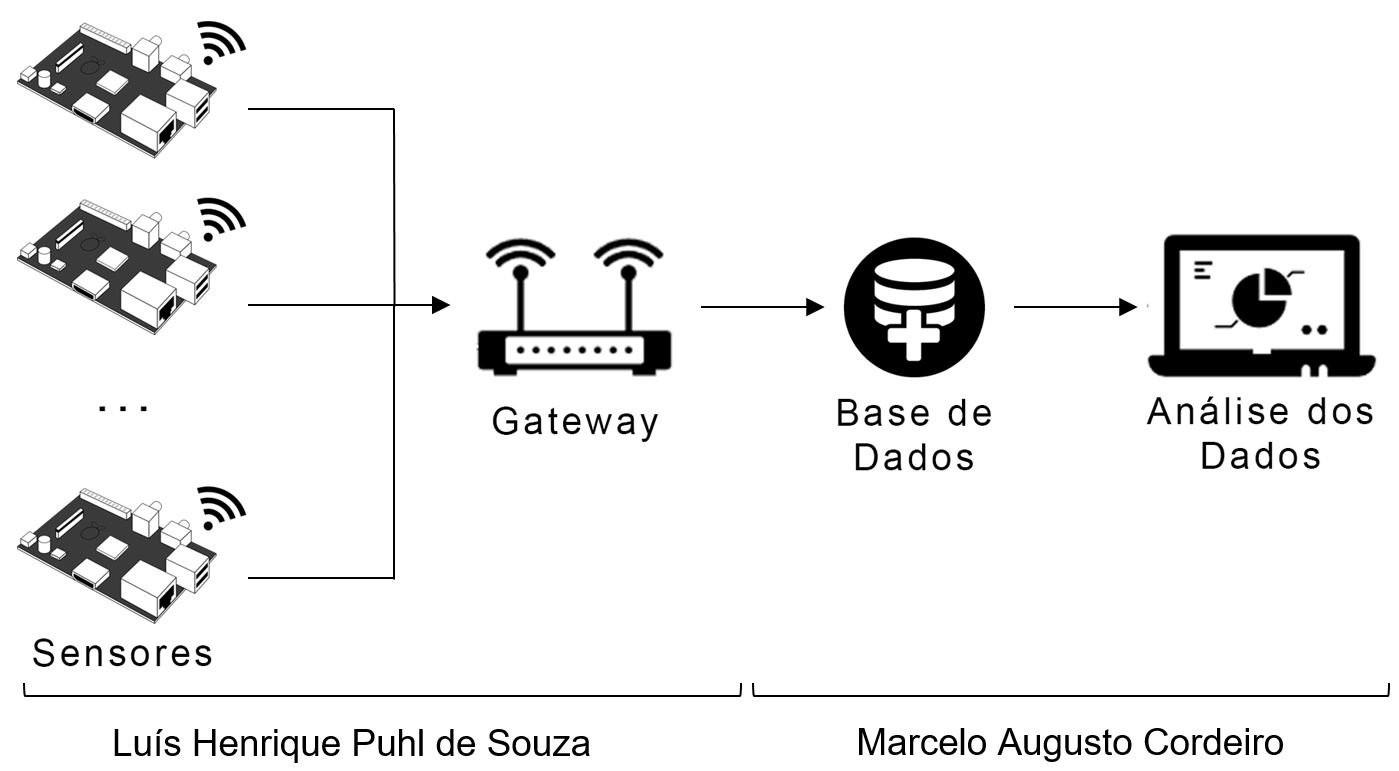
\includegraphics[width=1\textwidth]{030-justificativa/img/projeto.jpg}
	\end{center}
	\legend{Fonte: Marcelo Augusto Cordeiro \cite{Cordeiro2016}}
\end{figure}

A Figura \ref{fig:projeto} apresenta a arquitetura simplificada de uma aplicação
IoT, e no detalhe inferior a distribuição do desenvolvimento deste projeto IoT.

Para possibilitar testes em um ambiente real, o projeto aqui proposto será
instalado dentro do prédio do Laboratório de Tecnologia da Informação Aplicada
(LTIA) da Faculdade de Ciências da Unesp de Bauru.



\chapter{OBJETIVOS}
\label{chap:OBJETIVOS}

\section{OBJETIVO GERAL}
\label{sec:OBJETIVO GERAL}

Considerando características locais, propõem-se a construção de uma aplicação
para localizar contextualmente dispositivos dentro de um prédio piloto e avaliar
sua precisão.

Além desta aplicação, é objetivo definir o custo do projeto piloto, incluindo
esforço de pesquisa assim como definir um custo para replicação deste
localizador contextual em outros prédios utilizando como fonte de ferramentas e
recursos o mercado local.

\section{OBJETIVOS ESPECÍFICOS}
\label{sec:OBJETIVOS ESPECÍFICOS}

\begin{alineas}

	\item Estabelecer o estado da arte sobre a desenvolvimento de aplicações IoT;

	\item Identificar desafios locais para o desenvolvimento;

	\item Identificar provedores de serviços, dispositivos e ferramentas para o
desenvolvimento;

	\item Construir sensores de identificação e localização (distância) de
 dispositivos cuja comunicação seja baseada em \textit{Wi-Fi};

	\item Posicionar estes sensores;

	\item Construir um dispositivo agregador de informações dos sensores
 (\textit{gateway}) e sua interface web (Web REST API - \textit{Representational
State Transfer} \textit{Application Programming Interface});

	\item Estimar o custo total do projeto piloto incluindo esforço de pesquisa;

	\item Estimar o custo de replicação da aplicação em outros prédios
	utilizando fontes do mercado local.

\end{alineas}


\chapter{Fundamentação teórica}
\label{chap:Fundamentação teorica}


Para conceituar, fundamentar e dar suporte teórico ao presente trabalho
apresentam-se nesta seção os tópicos e definições dos segmentos: IoT,
localização contextual de dispositivos e localização baseada em redes sem fio.

\section{Internet das coisas (IoT)}
\label{sec:INTERNET DAS COISAS (IOT)}

Uma das primeiras aplicações e definições de IoT foi feita por Kevin Ashton em
1999 para a \textit{Procter \& Gamble} (P\&G) \cite{ASHTON2009} e
simultaneamente no laboratório Auto-ID Labs no Instituto de Tecnologia de
Massachusetts (MIT - \textit{Massachusetts Institute of Technology}) utilizando
identificação por radio-frequência (RFID - \textit{radio-frequency
identification}) \cite{ATZORI2010, Friedemann2011} e desde então cresceu
ultrapassando o escopo da tecnologia RFID porém sempre com as premissas de ``uma
infraestrutura global para a Sociedade da Informação, habilitando serviços
avançados através da interconexão de coisas (físicas e virtuais) baseadas em
tecnologias, existentes e evolutivas, de informação e comunicação'' descrita por
\apudonline[p.~1, grifo e tradução
nossa]{Wortmann2015}{InternationalTelecommunicationUnion2012}.

Hoje em dia, quase qualquer tecnologia de comunicação acessível a computadores
pode ser utilizada como meio de comunicação entre dispositivos IoT, tornando
RFID mais uma, porém de grande importância, tecnologia info-comunicacional a
disposição das coisas para sua conexão. Esta gama de tecnologias possibilita uma
variedade equivalente de coisas conectadas. Se a coisa pode usar de uma
tecnologia de conexão, considerando suas restrições de volume, custo e
utilidade, muito provavelmente vai fazê-lo gerando ao menos uma identidade
virtual representando seu objeto físico e seus atributos. Esta identidade
virtual e atributos virtuais serão expostos para todos indivíduos, humanos ou
coisas, que lhe forem convenientes de qualquer lugar do universo virtual,
fazendo efetivamente parte da internet.

\section{Localização contextual de dispositivos}
\label{sec:Localização contextual de dispositivos}

Em ciência da computação, os termos \textit{"Contexto"} e \textit{"Consciência
de Contexto"} expressam uma ideia recente estudada nos campos de inteligência
artificial e ciência cognitiva desde 1991. O tema "Contexto" ainda é considerado
atual e promissor a ponto de mudar o cenário de negócios nos próximos 10 anos
porém sem definição simples. Tamanha é a falta de uma definição geral que
realmente funcione para casos reais que existe uma proposta de definir o termo
utilizando uma nova metodologia de pesquisa holística através de mineração e
agrupamento de texto advindo de publicações cientificas \cite{Pascalau2013}.

Mesmo sem uma definição permanente em vista, utilizaremos o que é considerado
estado da arte para o termo \textit{"Contexto"} que foi introduzido por
\citeonline{Dey1999} e reforçado por \citeonline{Dey2000}:

\begin{citacao}

	``Contexto é qualquer informação que pode ser utilizada para caracterizar a
	situação de uma entidade. Uma entidade é uma pessoa, lugar ou objeto que é
	considerado relevante para a interação entre um usuário e uma aplicação,
	incluindo o próprio usuário e a aplicação.'' \

	\citeonline[p.~3]{Dey1999} Tradução Nossa.
\end{citacao}

\subsection{Localização contextual}
\label{subsec:Localização contextual}

Das informações contextuais que uma aplicação de cliente móvel pode obter, a
localização é uma das mais importantes. Ajudar pessoas a navegar por mapas,
encontrar objetos e pessoas com os quais tem interesse de interagir é sem dúvida
uma boa meta a ser alcançada com a coleta da localização do cliente
\cite{Bellavista2008}.

Na categoria de Serviços Baseados em Localização (LBS - \textit{Location-Based
Services}) existem duas gerações. A primeira orientada a conteúdo que falhou,
pois a informação de localização era armazenada pela rede (que geralmetne era
administrada por uma empresa de telecomunicações), podendo até ser vendida pelo
provedor a terceiros, causando a sensação de \textit{Spam} (conteúdo não
solicitado) no usuário final ao receber conteúdo desta provedora. Já na segunda
geração, a posse da informação foi movida para o cliente móvel, deixando a cargo
do usuário escolher se ela seria compartilhada e com quem. Esta mudança trouxe
maior engajamento do usuário, resultando numa maior aceitação dessa geração
\cite{Bellavista2008}.


Ao contrário das técnicas atuais, neste trabalho os humanos ou tomadores de
decisão não estarão em posse do cliente móvel, e sim em posse do prédio.
Portanto, a mesma informação, sem degradação em sua importância, passará a ser
coletada e armazenada pelo provedor da rede como nos LBSs de primeira geração.
Esta decisão garante o foco no usuário uma vez que este mudou, antes ele detinha
um cliente móvel, agora ele detem múltiplos. Isso torna a detenção do todo
(coisas dentro do prédio) mais precioso do que o das partes (os clientes móveis)
além da mudança da propriedade da rede para o usuário final, na comparação
celular \textit{versus} \textit{Wi-Fi}.

Uma vez encontrada a localização de um dispositivo, metadados sobre o prédio são
mesclados formando um conjunto rico contextualmente do ponto de vista da
aplicação IoT Prédio como fornecedora principal dos dados para a internet e
portanto seus usuários detentores. Essa riqueza é garantida com metadados sobre
o dispositivo (identificação, nome, histórico, carecteristicas) e sobre o prédio
(ex.: mapa, estrutura de salas, horário de funcionamento, consumo energético,
humanos responsáveis e lista de equipamentos) que trazem possibilidades de
extração de informação importantes para os detentores deste prédio e seu
conteúdo. Esta capacidade do prédio deve-se pelo papel de coordenador de
informações e controlador de meta-informações semelhante ao Coordenador em uma
aplicação na arquitetura Modelo-Apresentação-Adaptador-Controlador-Coordenador
(MPACC - \textit{Model-PresentationAdapter-Controller-Coordinator}) proposto por
\citeonline{Roman2001}.


\subsection{Contexto de um dispositivo em um prédio}
\label{subsec:Contexto de um dispositivo em um prédio}

Para os metadados agregados à informação de posição pelo prédio definimos que o
modelo de divulgação terá de conter além da posição do dispositivo informação
sobre este (nome, histórico), informação da estrutura do prédio (mapa imagem,
mapa lógico, nome, localização global, endereço, etc), ligação entre a estrutura
do prédio e a localização do dispositivo (posição no mapa lógico) e informação
sobre o estado do prédio (horário de funcionamento, frequentadores, etc).


Este modelo visa prover fácil mineração e reutilização de informações por
terceiros após a implementação do projeto que é medida pela disponibilidade e
relacionamento das informações providas. Essa métrica também será utilizada para
avaliar o projeto final.

Este foco em reusabilidade vem da definição de Web Semantica (\textit{Semantic
Web}) e de uma de suas realizadoras, a Ligação de Dados (\textit{Linked Data}),
que sugerem o uso de um formato padrão além de ser acessível e gerenciável pelas
ferramentas de exploração. Desta forma a Web de Dados (\textit{Web of Data}) é
construída opondo uma simples coleção de dados \cite{Bizer2009}.

\section{Localização baseada em redes sem fio}
\label{sec:Localização baseada em redes sem fio}

Para o sistema de posicionamento nos baseamos em técnicas de
\textit{n-lateração?} de distâncias adquiridas com a medição de características
eletromagnéticas (ex.: potência de sinal) e dos protocolos (ex.: Tempo de
chegada) que já foram explorados anteriormente \cite{Abusubaih2007,
bahillo2009ieee, Feldmann2003}.

Portanto os sensores seguirão as especificações de \textit{WiFi IEEE 802.11}
\cite{Crow1997} e técnicas definidas para \textit{Bluetooth Low Energy (BLE)}
\cite{Hossain2007} devido a semelhança da área de cobertura (até 100 metros,
geralmente utilizado até 20 metros) e frequência (no caso de 2.4GHz).

Para construir estes sensores uma plataforma de hardware adequada é necessária,
para esta escolhemos o Raspberry Pi \cite{Vujovic2014, Vujovic2015} que já
foi provado funcional no caso de Localização através \textit{Wi-Fi} por
\citeonline{Ferreira2016} especialmente a sua versão 3 que adiciona a capacidade
de sensor \textit{Wi-Fi} e \textit{Bluetooth} em sua placa principal sem
necessidade de adaptadores externos destacando ainda mais sua escolha
\cite{RPI2016}.

Em adição, na construção dos sensores é testada a plataforma ESP-8266 bem como
outras alternativas que demonstrarem afinidade com o projeto não limitando as
escolhas durante o projeto a aquelas mencionadas na proposta original.



\chapter{MÉTODO DE PESQUISA}
\label{chap:MÉTODO DE PESQUISA}

Abordagens para medir distâncias através de redes sem fio \textit{Wi-Fi}
\cite{bahillo2009ieee} e \textit{Bluetooth} já existem e, propor novas maneiras
não é o foco deste trabalho. Utilizando essas técnicas, estabelece uma
rede de nós sensores colaborativos fixos no ambiente onde deseja-se obter a
localização dos dispositivos. As informações de distância serão compartilhadas
entre os nós para maior precisão da informação.

Para a implementação, pretende-se utilizar os \textit{softwares} de maior
destaque recentemente nos ramos de comunicação de baixa energia (\textit{MQTT}),
serviços \textit{Web} para armazenamento (\textit{MongoDB}) e publicação
(\textit{NodeJS}), além de \textit{softwares} para medição da distância sem
interferir na comuncação (\textit{Sniffing}) e das plataformas de
\textit{hardware} disponíveis e recomendadas para IoT com capacidade
\textit{Wi-Fi} (\textit{Raspberry Pi 3} e \textit{ESP-8266}).

Mesmo com a grande quantidade de dispositivos já conectados são poucos os
documentos descrevendo boas práticas para concepção, construção e manutenção de
aplicações IoT, especialmente sobre os cuidados tomados quanto a segurança e
análise de custos para a implementação e manutenção.

Além disso, a falta de referências neste sentido é agravada quando considera-se
a implementação no interior do estado de São Paulo. Nesta região, poucas são as
organizações atualizadas neste tema, levando a uma falta enorme de conteúdo
escrito na linguagem local além de serviços e produtos disponíveis para
construção de uma plataforma completa e competitiva nesta região.

Devido a falta de conteúdo e instrução, utiliza-se prototipagem ágil neste
projeto, uma vez que esta metodologia de desenvolvimento é recomendada para
projetos cujas especificações e definições não são claras, demandando muitas
modificações das mesmas durante a execução do projeto. Esse método entra em
contraste com metodologias clássicas, como a cascata que apesar de previsíveis,
não reagem bem a ambientes de extrema incerteza.

Mais especificamente, utiliza-se uma variante da metodologia \textit{Scrum}
\cite{James2016} que será adaptada para o projeto. Nela, serão executadas
iterações de uma semana em que a cada iteração, uma nova versão melhorada do
produto completo (\textit{hardware}, \textit{software}, documentação e
resultados) é entregue.

Dentro de cada iteração, as camadas da aplicação IoT serão escolhidas,
implementadas, justificadas e avaliadas, sendo todo processo documentado. Como
resultado de cada uma delas, será gerado um relatório das mudanças a partir da
iteração anterior.

Com mais detalhes, cada iteração cumprirá uma parte de cada objetivo no trabalho
completo levando o projeto integralmente para um estágio de completude maior a
cada iteração. Serão foco de cada iteração os objetivos abaixo, gerando um
relatório utilizado para tomar e justificar decisões durante a execução do
projeto bem como servir de posterior documentação. Os objetivos de cada iteração
são:

\begin{alineas}

	\item Escolha de provedores de serviços, dispositivos e ferramentas para o
desenvolvimento;

	\item Construir, avaliar, testar e manter os sensores;

	\item Construir o dispositivo agregador e sua API;

	\item Estimar o custo total do projeto piloto;

	\item Estimar o custo de replicação;

	\item Identificar os desafios para o desenvolvimento.

\end{alineas}

Desta forma, espera-se garantir a liberdade necessária para o projeto ser
executado com sucesso, mesmo no ambiente de incerteza no qual o mercado local de
IoT encontra-se, cumprindo as premissas de de funcionamento, manutenção e
segurança que são grande importância para os interessados na área.



\chapter{CRONOGRAMA}
\label{chap:CRONOGRAMA}

Devido a natureza ágil e iterativa da metodologia, o cronograma será dividido em
apenas três partes: Levantamento Bibliográfico Inicial, Desenvolvimento
Iterativo (Escolha de provedores e fornecedores; Construção, avaliação, teste e
manutenção dos sensores e agregadores; Estimativas de custos totais e de
replicação e Documentação de desenvolvimento) e Revisão Final. Estas partes
serão distribuídas durante o ano letivo conforme a Tabela 1 considerando as
alterações do calendário letivo da Faculdade de Ciências da UNESP de Bauru que
esteve em estado de greve de 1º de Junho à 18 de Agosto de 2016.

\begin{table}[htb]
\IBGEtab{%
\ABNTEXchapterfont {
  \caption{Cronograma de Atividades Propostas}%
  \label{table:cronograma}
}
}{%
  \begin{tabular}{cccccccccccc}
  \toprule
	Atividade															&	Fev	&	Mar	&	Abr	&	Mai	&	Ago	&	Set	&	Out	&	Nov	&	Dez	&	Jan	&	Total	\\
  \midrule \midrule
	Levantamento Bibliográfico \\ Inicial								&	X	&	X	&	 	&	 	&	 	&	 	&	 	&	 	&	 	&		&	2	\\
	\midrule
	Escolha de \\ provedores e fornecedores								&	 	&	X	&	X	&	X	&	X	&	X	&	X	&		&		&		&	6	\\
	\midrule
	Construção, avaliação e\\manutenção  dos sensores \\ e agregadores	&	 	&		&	X	&	X	&	X	&	X	&	X	&	X	&		&		&	6	\\
	\midrule
	Estimativas de custos												&	 	&		&		&		&	X	&	X	&	X	&	X	&	X	&		&	5	\\
	\midrule
	Documentação de \\ desenvolvimento									&	 	&		&	X	&	X	&	X	&	X	&	X	&	X	&	X	&		&	7	\\
	\midrule
	Revisão Final														&	 	&	 	&	 	&	 	&	 	&	 	&	 	&	X 	&	X	&	X	&	3	\\
	\midrule \midrule
	Semanas disponíveis													&	4 	&	5 	&	4 	&	4 	&	2 	&	 4	&	4 	&	4 	&	3	&	3	&	37	\\
	\midrule
	Total de atividades													&	4 	&	10 	&	12 	&	12 	&	8 	&	 16	&	16 	&	16 	&	9	&	3	&	106	\\
	\midrule
	\bottomrule
\end{tabular}%
}{%
  \fonte{Produzido pelo autor.}%
  }
\end{table}

Cada atividade realizada representa uma melhoria ou avanço no projeto total
porém o número total é apenas uma estimativa devido a natureza da metodologia.
Nesta segunda versão do cronograma foram estimadas 106 atividades distribuidas
em 37 semanas, de acordo com as alterações dos calendários letivos anteriormente
mencionados. As diferenças entre as duas vesões são nos meses de junho a janeiro
onde houve redução de 40 para 37 semanas disponíveis e consequente redução da
estimativa de atividades de 111 para 106.



% ----------------------------------------------------------------------------

% ELEMENTOS PÓS-TEXTUAIS

% Referências bibliográficas
\bibliography{900-referencias/referencias}


\ifglossario
	Glossário
\fi

\ifapendice
	Apêndice de meu desenvolvimento.
\fi

\ifanexo
	Anexo de outros autores.
\fi

\ifindice
	Indice Remissivo
\fi

\end{document}
